\documentclass[aspectratio=169]{beamer}
\usepackage[utf8]{inputenc}
\usepackage{tikz} % for QR code overlay

% code snippets
\usepackage{minted}
\newmintedfile[dockercode]{dockerfile}{
  % bgcolor=mintedbackground,
  fontfamily=tt,
  linenos=true,
  numberblanklines=true,
  numbersep=5pt,
  gobble=0,
  frame=leftline,
  framerule=0.4pt,
  framesep=2mm,
  funcnamehighlighting=true,
  tabsize=4,
  obeytabs=false,
  mathescape=false
  samepage=false, %with this setting you can force the list to appear on the same page
  showspaces=false,
  showtabs =false,
  texcl=false,
}
\newminted[bashcode]{bash}{
  % bgcolor=mintedbackground,
  fontfamily=tt,
  linenos=true,
  numberblanklines=true,
  numbersep=5pt,
  gobble=0,
  frame=leftline,
  framerule=0.4pt,
  framesep=2mm,
  funcnamehighlighting=true,
  tabsize=4,
  obeytabs=false,
  mathescape=false
  samepage=false, %with this setting you can force the list to appear on the same page
  showspaces=false,
  showtabs =false,
  texcl=false,
}

% biblatex (requires biber; sudo pacman -S biber)
\usepackage[]{biblatex} % biblatex
\addbibresource{./content/bib/bib1.bib}
\addbibresource{./content/bib/bib2.bib}
\addbibresource{./content/bib/throwaway.bib}

\usepackage{graphicx}
\graphicspath{ {./content/img/} }

\usetheme{Boadilla}
\usecolortheme{rose}
% \beamerdefaultoverlayspecification{<+->} % this will turn it into slides

\title{Privacy-Preserving Encrypted Deep Learning}
\subtitle{Artificial Intelligence}
\author{George Onoufriou\\(University of Lincoln)}
\date{\today}

\begin{document}

\addtobeamertemplate{frametitle}{}{%
\begin{tikzpicture}[remember picture,overlay]
\node[anchor=north east,yshift=2pt] at (current page.north east) {
\includegraphics[height=1.5cm]{qrcode.png}};
\end{tikzpicture}}

  \frame{\titlepage}

  \begin{frame}
    \frametitle{About}
    \begin{columns}
      \begin{column}{0.5\textwidth}
        \begin{itemize}
          \item PhD Candidate Computer/ Data Science
          \item Privacy and Linux Enthusiast
        \end{itemize}
      \end{column}
      \begin{column}{0.5\textwidth}
        \begin{figure}[th!]
          \centering
          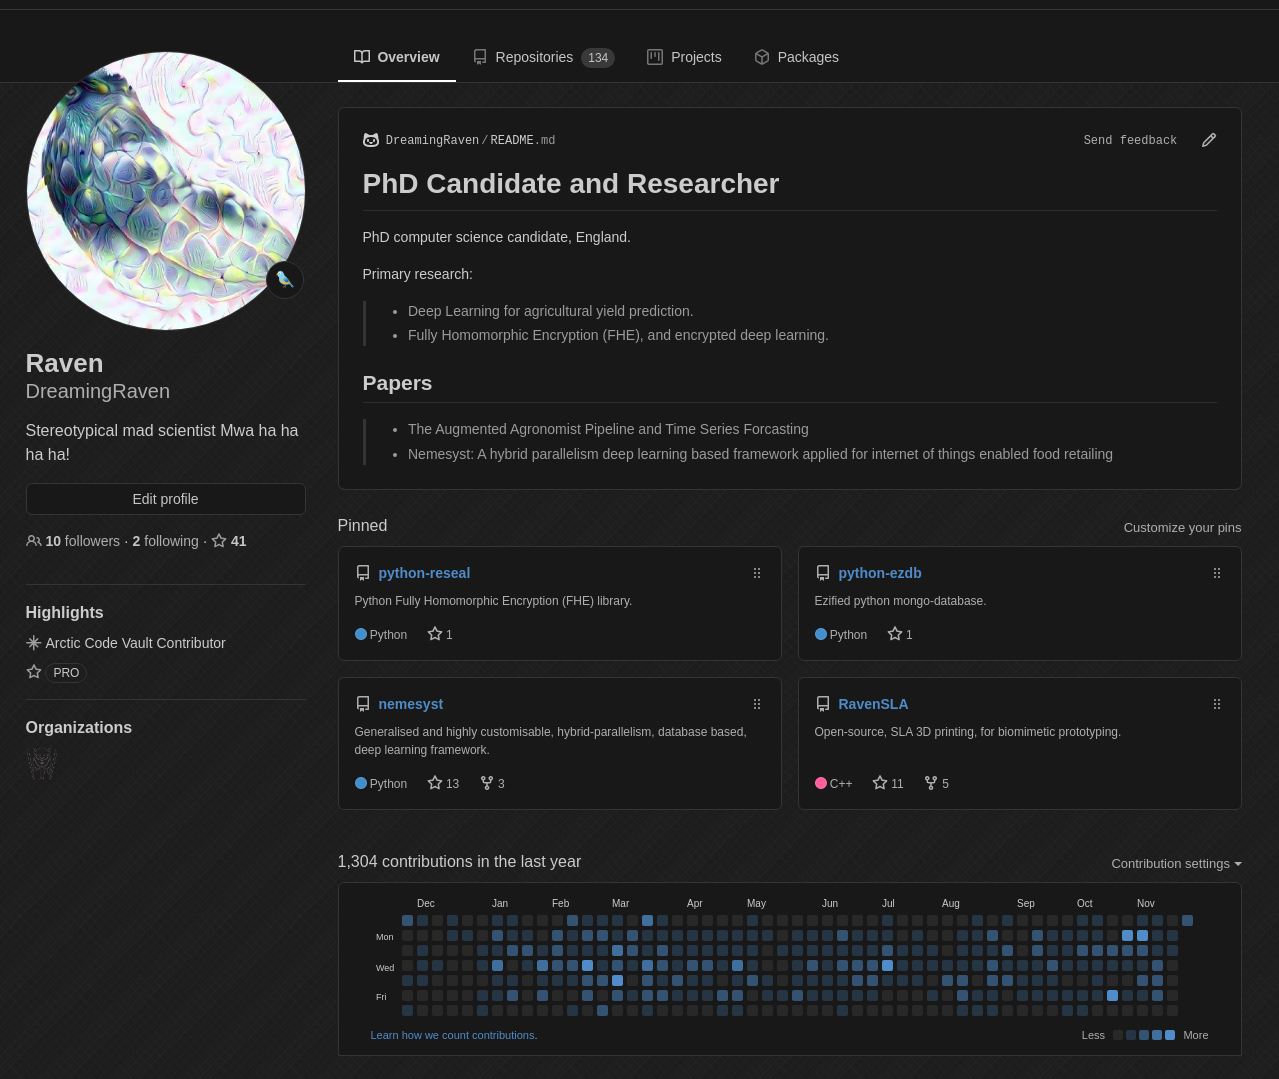
\includegraphics[width=0.8\textwidth]{gh.png}
          \caption{GitHub profile page where you can come to see my work and chat. \autocite{repository}}
          \label{fig:gh}
        \end{figure}
      \end{column}
    \end{columns}
  \end{frame}

  \begin{frame}
    \frametitle{My Work}
    \begin{columns}
      \begin{column}{0.5\textwidth}
        I work with:
        \begin{itemize}
          \item Deep Learning (subfield of Artificial Intelligence, and probably the coolest part of AI)
          \item Fully Homomorphic Encryption
        \end{itemize}
        Applied to:
        \begin{itemize}
          \item Agriculture; Predicting plant yield, in particular strawberries.
        \end{itemize}
      \end{column}
      \begin{column}{0.5\textwidth}
        \begin{figure}[th!]
          \centering
          \includegraphics[angle=-90,origin=c,width=0.55\textwidth]{wasp.jpg}
          \caption{Strawberry tabletop with a wasp having some lunch.}
          \label{fig:wasp}
        \end{figure}
      \end{column}

    \end{columns}
  \end{frame}

  \begin{frame}
    \frametitle{What is Artificial Intelligence}
    \begin{columns}
      \begin{column}{0.5\textwidth}
        \begin{itemize}
          \item T-800 coming for John Connor?
        \end{itemize}
      \end{column}
      \begin{column}{0.5\textwidth}
        \begin{figure}[th!]
          \centering
          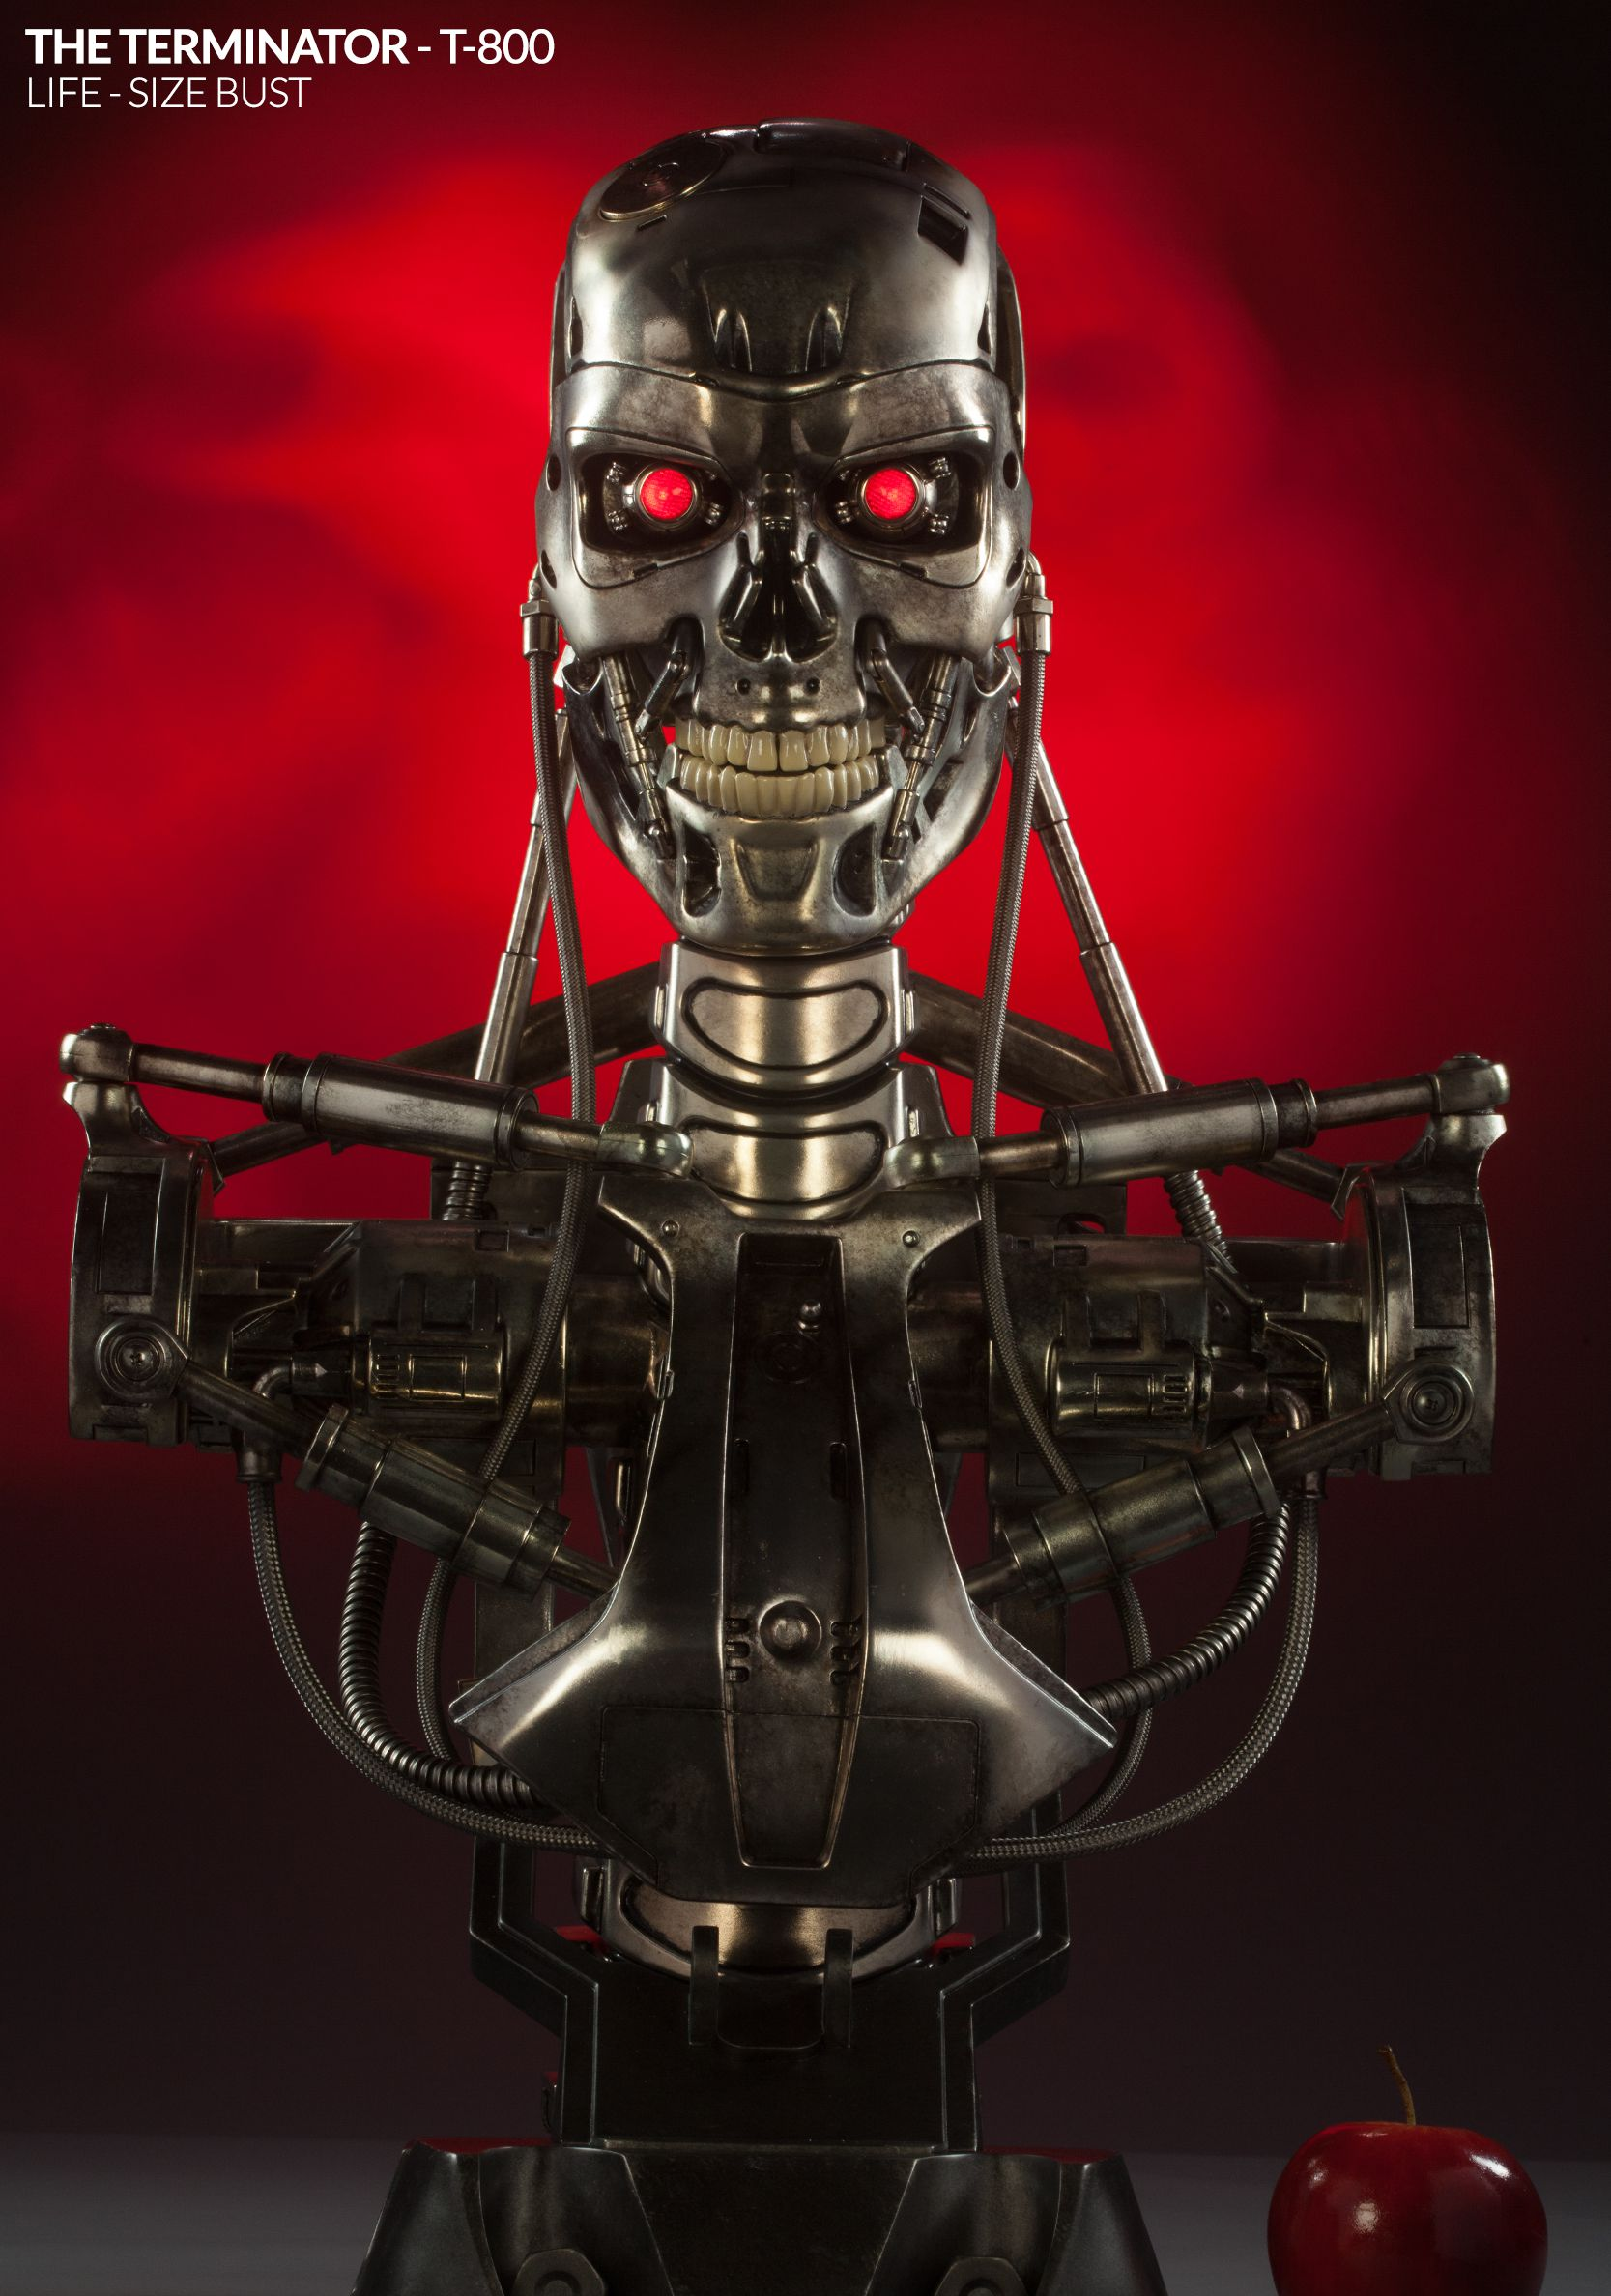
\includegraphics[width=0.5\textwidth]{t800.jpg}
          \caption{T-800, terminator bust from sideshow collectibles.}
          \label{fig:jim_carrey}
        \end{figure}
      \end{column}
    \end{columns}
  \end{frame}

  \begin{frame}
    \frametitle{What is Artificial Intelligence}
    \begin{columns}
      \begin{column}{0.5\textwidth}
        \begin{itemize}
          \item HAL9000?
        \end{itemize}
        Who in both the film and novel is capable of:
        \begin{itemize}
          \item Speech/ speech recognition, known as natural language processing (NLP)
          \item Facial recognition
          \item Lip reading
          \item Art appreciation
          \item Playing chess
        \end{itemize}
      \end{column}
      \begin{column}{0.5\textwidth}
        \begin{figure}[th!]
          \centering
          
\includegraphics[width=0.2\textwidth]{hal9000.pdf}
          \caption{HAL9000, Space Odyssey. Image by Grafiker61}
          \label{fig:jim_carrey}
        \end{figure}
      \end{column}
    \end{columns}
  \end{frame}

  \begin{frame}
    \frametitle{What is Artificial Intelligence}
    \begin{columns}
      \begin{column}{0.5\textwidth}
        Who in both the film and novel is capable of:
        \begin{itemize}
          \item Speech/ speech recognition, known as natural language processing (NLP)
          \item Facial recognition
          \item Lip reading
          \item Art appreciation
          \item Playing chess $+$
        \end{itemize}
      \end{column}
      \begin{column}{0.5\textwidth}
        \begin{figure}[th!]
          \centering
          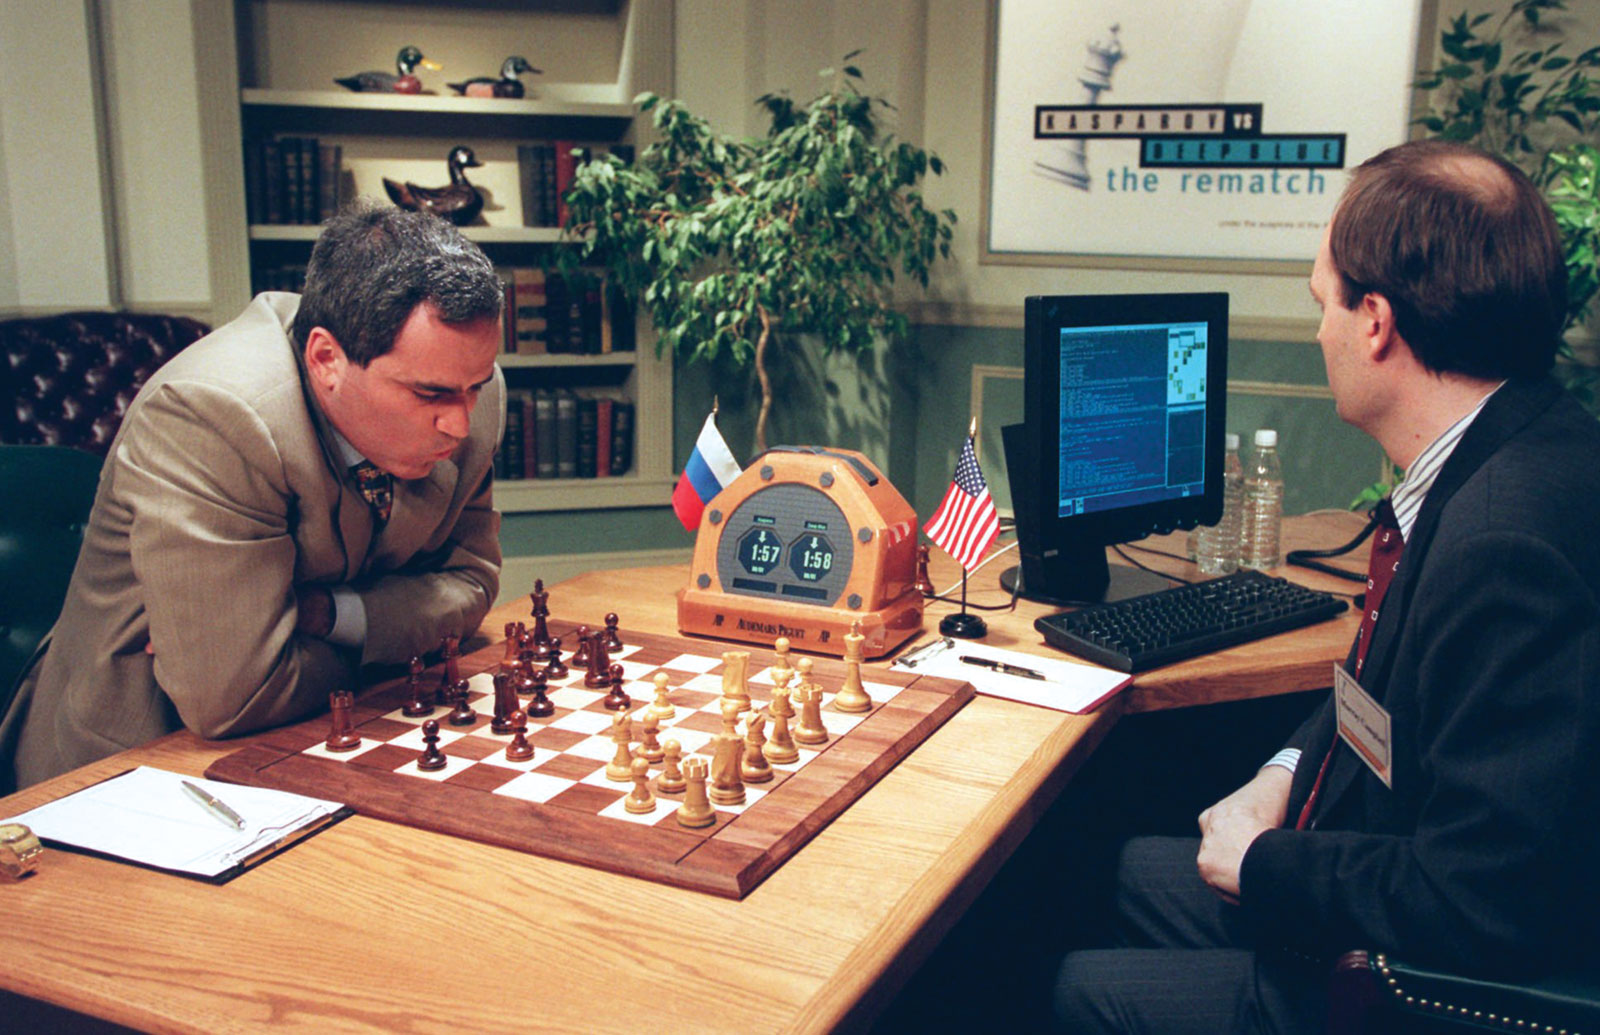
\includegraphics[width=1\textwidth]{deep-blue.jpg}
          \caption{Deep Blue beating world champion Garry Kasparov on their first game (1996)}
          \label{fig:jim_carrey}
        \end{figure}
      \end{column}
    \end{columns}
  \end{frame}

  \begin{frame}
    \frametitle{What is Artificial Intelligence}
    \begin{columns}
      \begin{column}{0.5\textwidth}
        Who in both the film and novel is capable of:
        \begin{itemize}
          \item Speech/ speech recognition, known as natural language processing (NLP) $+$
          \item Facial recognition
          \item Lip reading
          \item Art appreciation
          \item Playing chess
        \end{itemize}
      \end{column}
      \begin{column}{0.5\textwidth}
        \begin{figure}[th!]
          \centering
          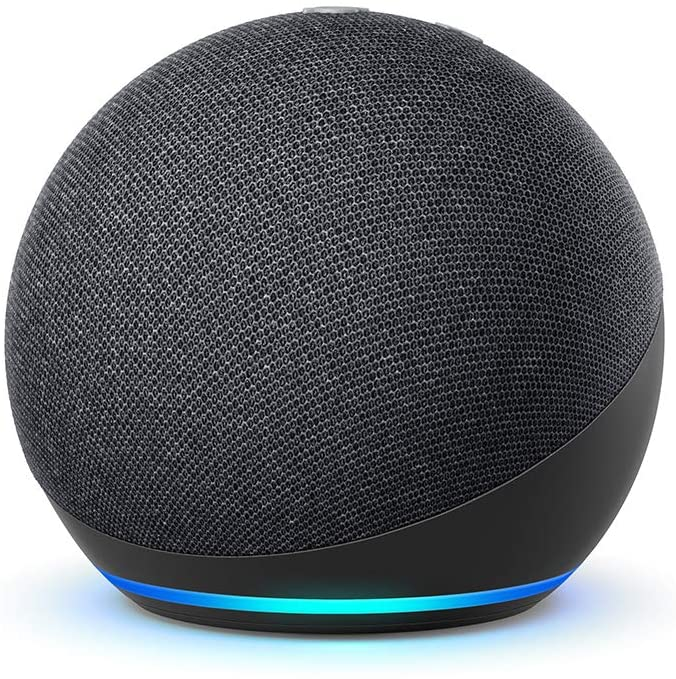
\includegraphics[width=0.5\textwidth]{alexa.jpg}
          \caption{Amazon Alexa, echo dot gen 4}
          \label{fig:jim_carrey}
        \end{figure}
      \end{column}
    \end{columns}
  \end{frame}

  \begin{frame}
    \frametitle{What is Artificial Intelligence}
    \begin{columns}
      \begin{column}{0.5\textwidth}
        Who in both the film and novel is capable of:
        \begin{itemize}
          \item Speech/ speech recognition, known as natural language processing (NLP)
          \item Facial recognition
          \item Lip reading
          \item Art appreciation $-$
          \item Playing chess
        \end{itemize}
      \end{column}
      \begin{column}{0.5\textwidth}
        \begin{figure}[th!]
          \centering
          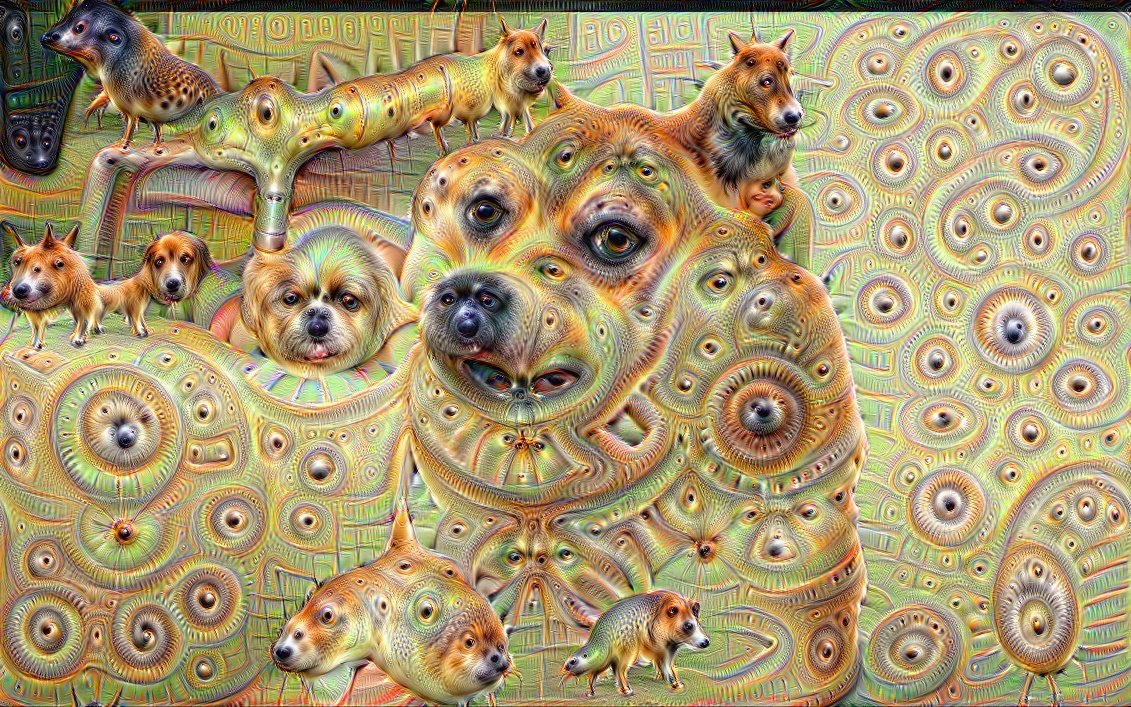
\includegraphics[width=0.9\textwidth]{deep-dream.jpg}
          \caption{Google Deep Dream Generator}
          \label{fig:jim_carrey}
        \end{figure}
      \end{column}
    \end{columns}
  \end{frame}

  \begin{frame}
    \frametitle{What is Artificial Intelligence}
    \begin{columns}
      \begin{column}{0.9\textwidth}
        \begin{figure}[th!]
          \centering
          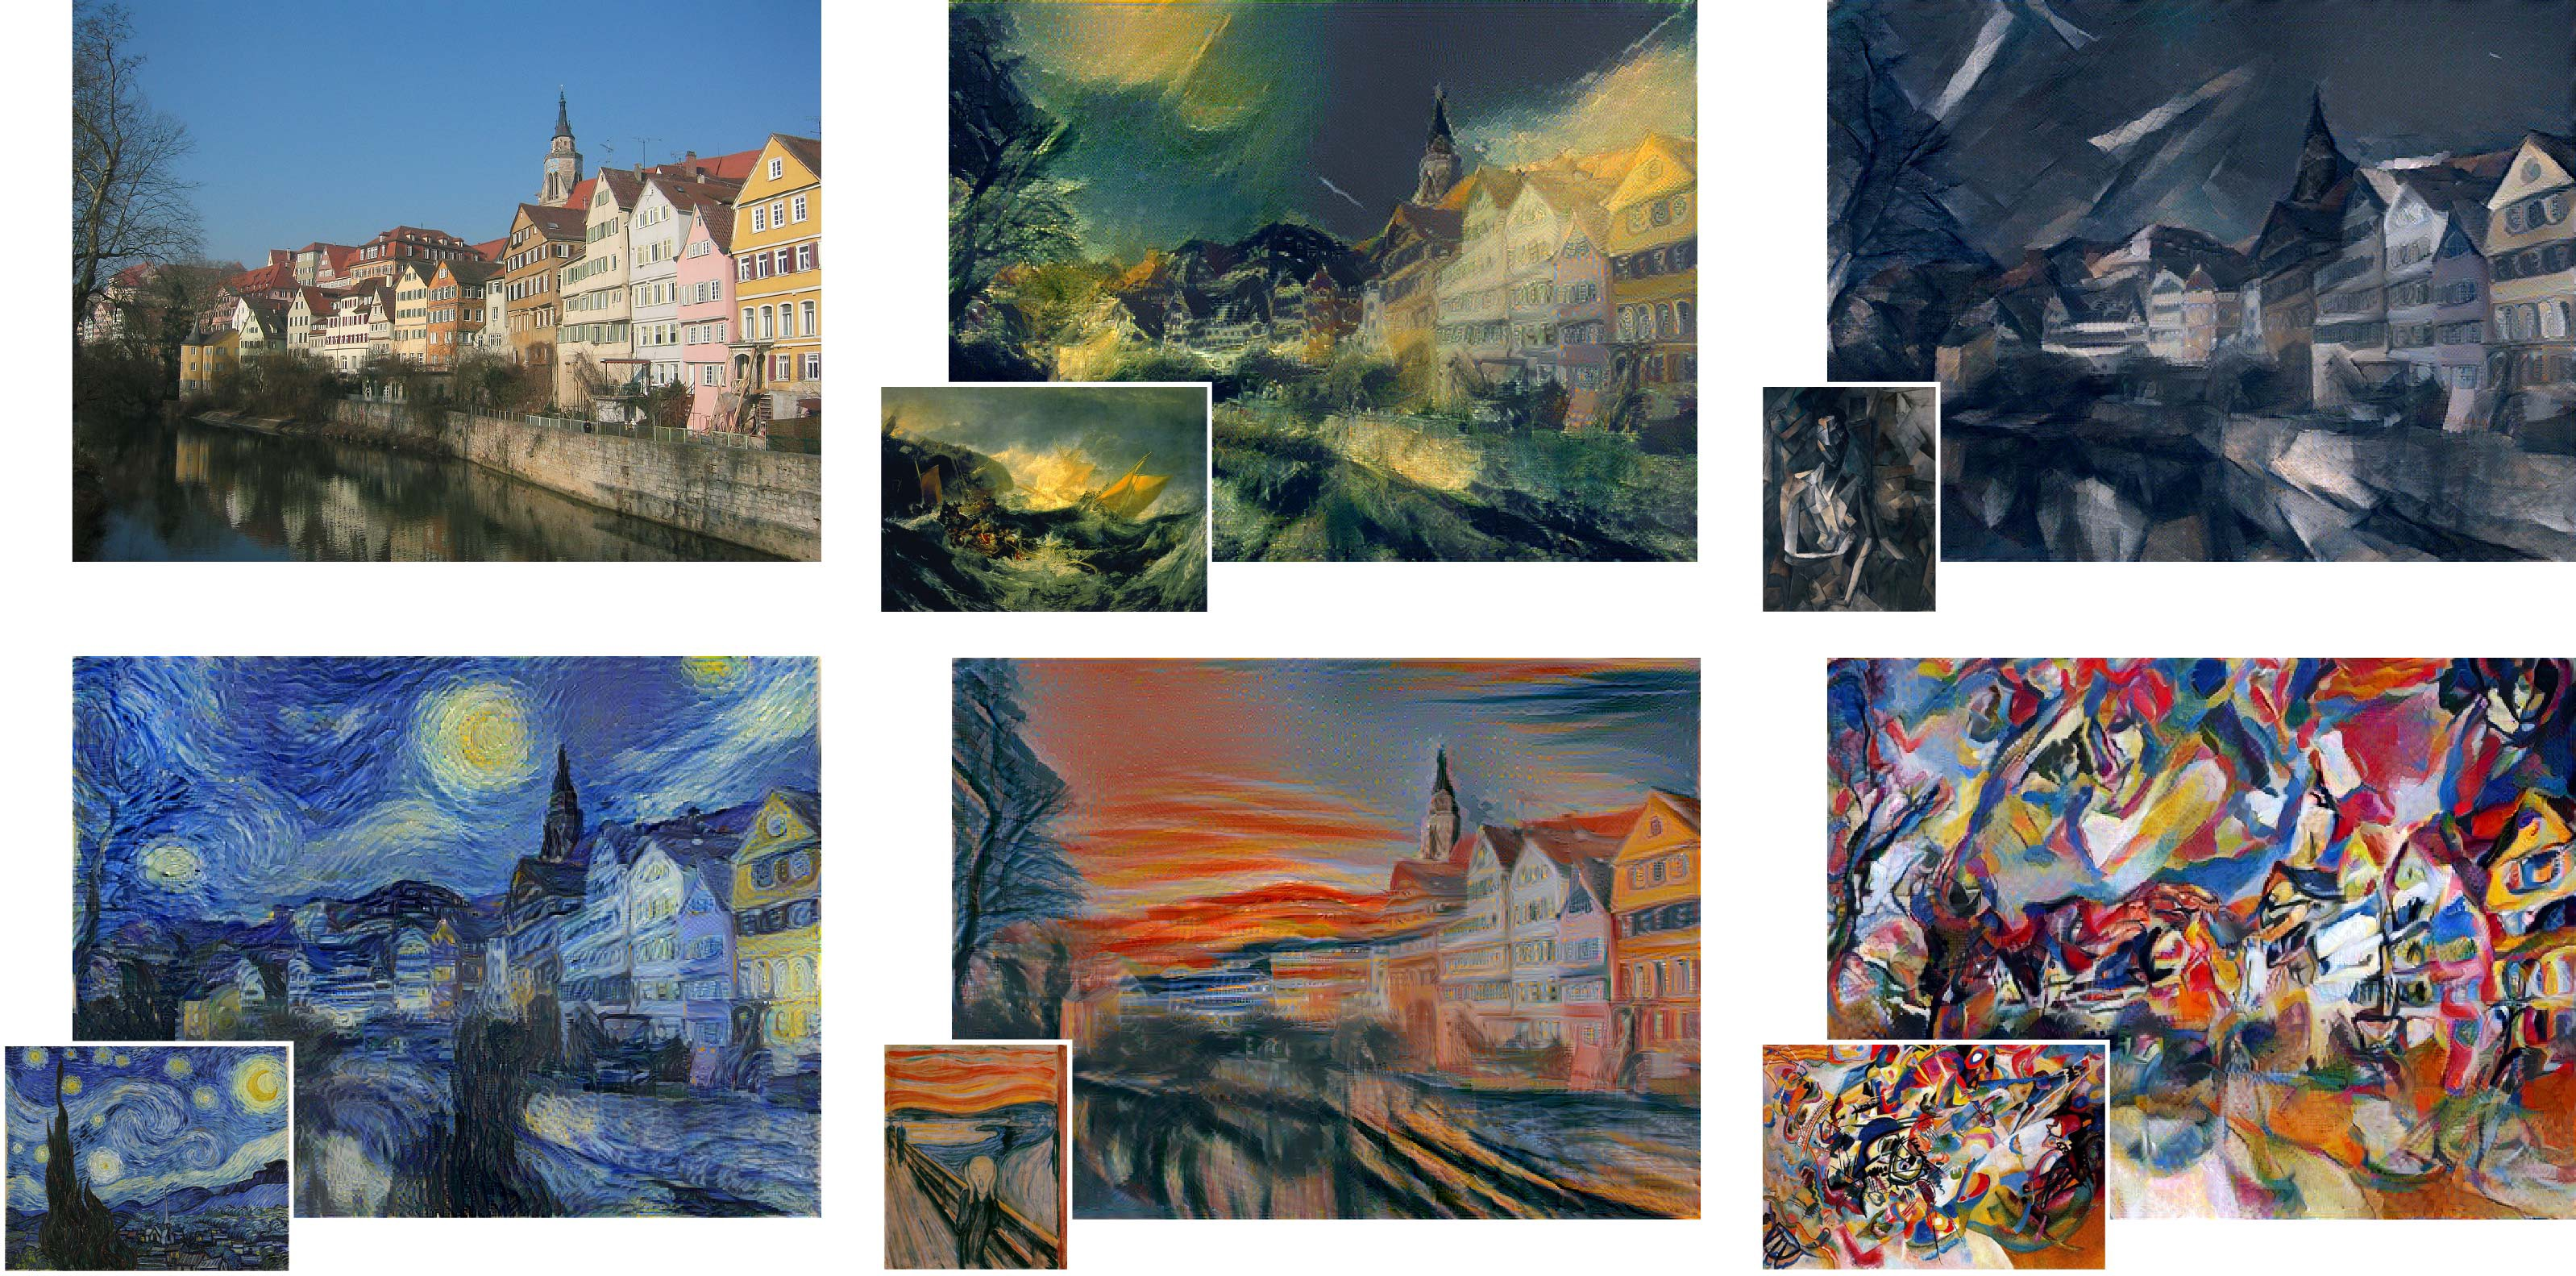
\includegraphics[width=0.9\textwidth]{style-transfer.jpeg}
          \caption{Deep Style Transfer}
          \label{fig:jim_carrey}
        \end{figure}
      \end{column}
    \end{columns}
  \end{frame}

  \begin{frame}
    \frametitle{Deep Learning and What Makes it Interesting}
    \begin{columns}
      \begin{column}{0.5\textwidth}
        \begin{itemize}
          \item Machines making sense of the world; Recognizing patterns
          \item (Pseudo) Artificial neurons, like you have in your brain
          \item We perceive things intuitively, but it is quite difficult for a machine
          \item Deep Learning is a set of cool techniques that can be transfered to many places
          \item State-of-the-art in almost every field it has been applied to
        \end{itemize}
      \end{column}
      \begin{column}{0.5\textwidth}
        \begin{figure}[th!]
          \centering
          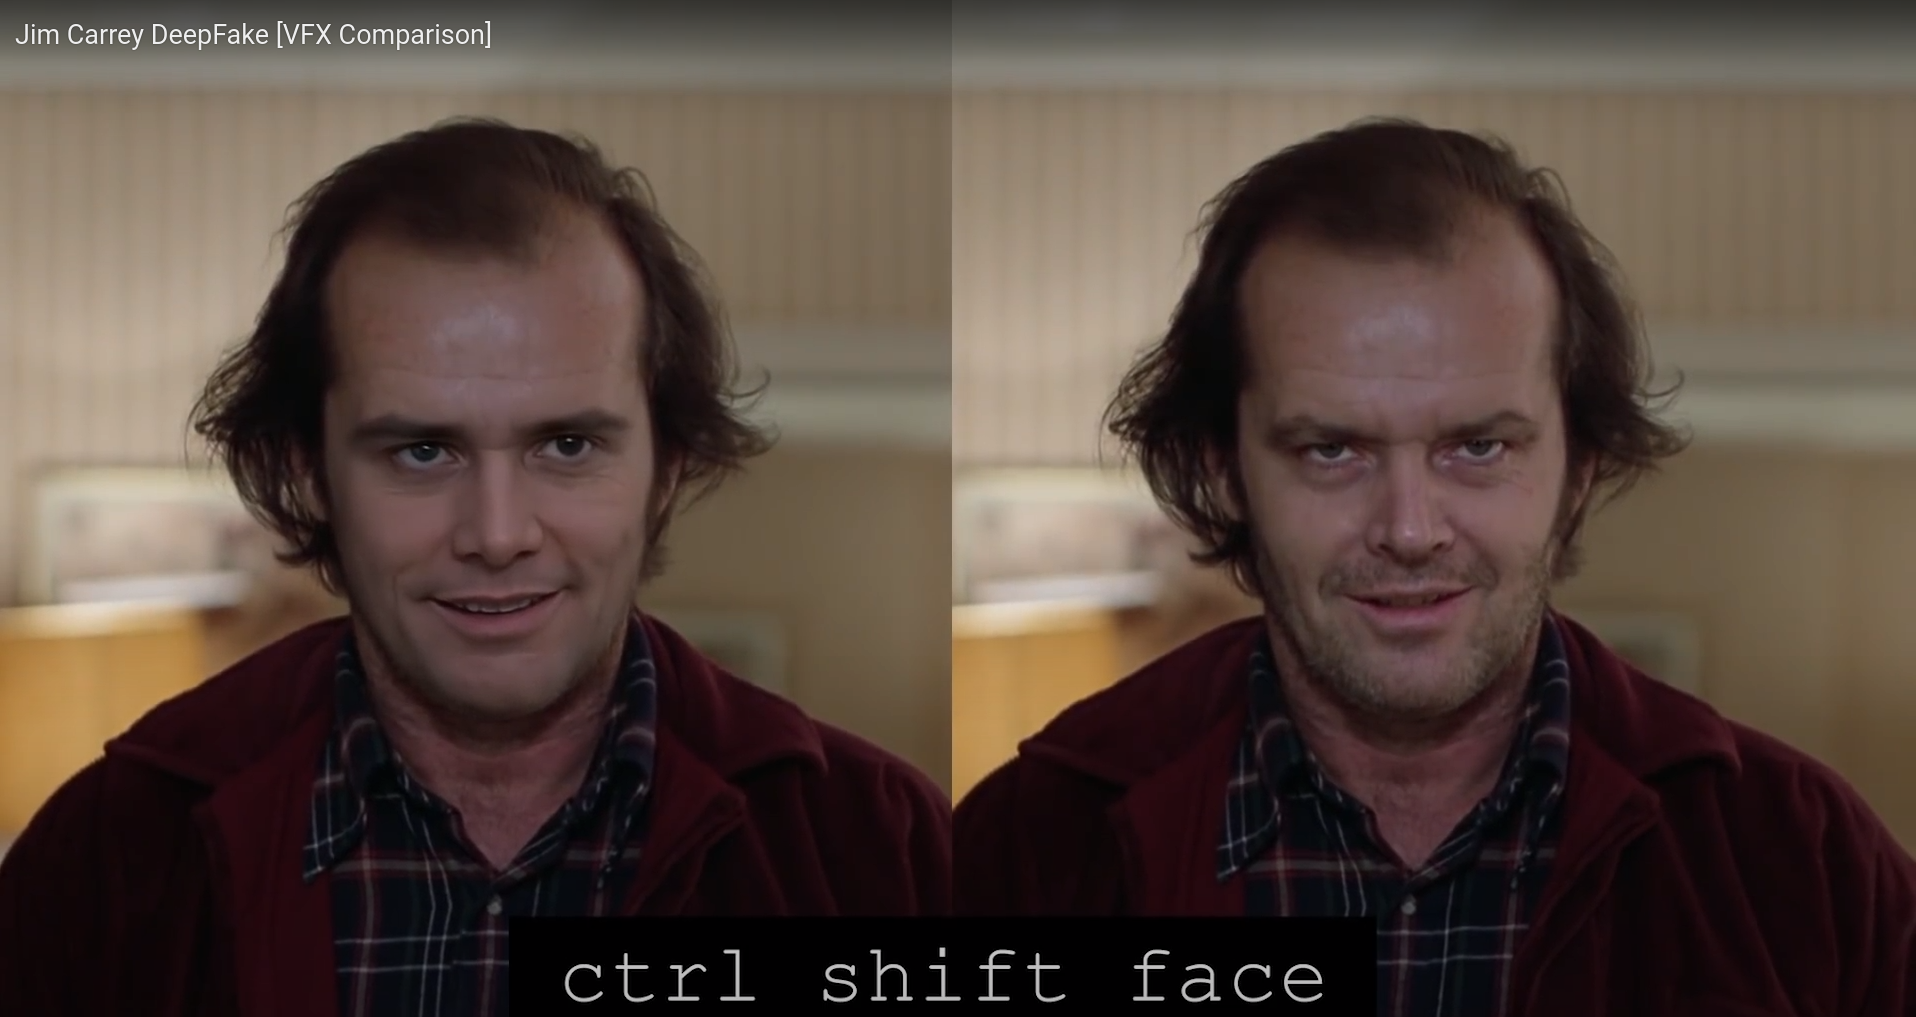
\includegraphics[width=1\textwidth]{jim_carrey.png}
          \caption{Jim Carrey (left) as Jack Nicholson (right), the shining deep fake.\autocite{deepfake}}
          \label{fig:jim_carrey}
        \end{figure}
      \end{column}
    \end{columns}
  \end{frame}

  \begin{frame}
    \frametitle{Fully Homomorphic Encryption and What Makes it Interesting}
    \begin{columns}
      \begin{column}{0.5\textwidth}
        \begin{itemize}
          \item Allows encrypted data to be added and multiplied with/to
          \item Gives us an alternative to protect sensitive data
          \item Simple yet achieves the otherwise impossible
          \item Use deep learning on something encrypted like diagnosis, and prediction with trade secrets
        \end{itemize}
      \end{column}
    \end{columns}
  \end{frame}

  \begin{frame}
    \frametitle{Interested?}
    \begin{columns}
      \begin{column}{0.5\textwidth}
        I got here through:
        \begin{itemize}
          \item A-Level, BSc Computer Science, PhD Computer Science
          \item Exploring the things that interested me
          \item Getting to know the people
        \end{itemize}
        Computer Science takes you places, as it is so broad.
      \end{column}
      \begin{column}{0.5\textwidth}
        Everyone is different you might go a different route:
        \begin{itemize}
          \item Computer science can be learned easily by anyone with a reasonable computer and internet connection for free
        \end{itemize}
        Good places to start are:
        \begin{itemize}
            \item Deep Learning by Goodfellow et al \autocite{Goodfellow-et-al-2016}
            \item Coursera deep learning specialisation
            \item Andrej Karpathy's youtube series on deep learning
        \end{itemize}
      \end{column}
    \end{columns}
  \end{frame}

  \begin{frame}
    \frametitle{Summary}
    \begin{columns}
      \begin{column}{0.5\textwidth}
        \begin{itemize}
          \item Introduce myself
          \item Introduce the problem of secrets
          \item What is deep learning
          \item What is fully homomorphic encryption
          \item How I got here
          \item How to find out more if it interests you
        \end{itemize}
      \end{column}
      \begin{column}{0.5\textwidth}
        \begin{figure}[th!]
          \centering
          \includegraphics[angle=-90,origin=c,width=0.6\textwidth]{strawberry.jpg}
          \caption{A strawberry for your time.}
          \label{fig:strawberry}
        \end{figure}
      \end{column}
    \end{columns}
  \end{frame}

  \begin{frame}[allowframebreaks]
    \frametitle{References}
    % % biblatex version
    \printbibliography
  \end{frame}

  \begin{frame}
      \frametitle{Questions}
      Come and ask questions!
      \url{https://github.com/DreamingRaven/encrypted-deep-learning-presentation}
  \end{frame}


\end{document}
